\chapter{Verification and Validation}
\label{ch:VerificationValidation}
Verification and Validation (V\&V) are essential steps in the design process to ensure that the design meets the requirements, and is free of errors.
To perform an informed trade-off in~\Cref{ch:TradeOff}, the preliminary sizing tool from~\Cref{ch:PrelimSizing} is verified and validated.
This chapter describes the verification (\Cref{sec:Verification}) and validation (\Cref{sec:Validation}) of the preliminary sizing tool and the concepts designed in~\Cref{ch:Concepts}, and provides recommendations for future V\&V in~\Cref{sec:VVProcedure}.

\section{Verification}\label{sec:Verification}
Verification of the preliminary sizing tool from~\Cref{ch:PrelimSizing} has been performed on a basic level, through unit tests for several functions within the model, and
a sensitivity analysis of the mass model.
Additionally, several equations were verified through various mathematical models, as well as the model that is verified with the requirements.








\subsection{Sensitivity Analysis}
A sensitivity analysis is performed on the mass model to check the sensitivity of the total mass to the different parameters, conducted by varying each parameter by 1\% and checking the effect on the total mass.
The results are shown in \Cref{tab:sensitivity-analysis}.
Moreover, the sensitivity analysis showed that the total mass is most sensitive to the estimated $C_{\text{D}_{\text{0}}}$, which means that for the detailed design phase, the drag coefficient should be calculated as accurately as possible.
Also, the total mass is very sensitive to the battery energy density, and some efficiency parameters.
These results are in line with the expectations, as the battery is a significant part of the total mass, and the efficiency of the propulsion system is crucial for energy consumption.


\begin{table}[H]
    \centering
    \caption{Sensitivity analysis of the mass model}
    \label{tab:sensitivity-analysis}
    \sisetup{table-format=+5.3, round-mode=figures, round-precision=3}
    \begin{tabular}{@{}l|Sc@{}}
        \toprule
        \textbf{Parameter}                 & \multicolumn{2}{|c}{\textbf{Total Mass Sensitivity}} \\
        \midrule
        Battery energy density             & -2095.726694891519      & [\unit{\kg^2\per\kWh}] \\
        Propeller radius                   &  -576.125257792963      & [\unit{\kg\per\m}] \\
        Take-off load factor               &   299.51798521836355    & [\unit{\kg}] \\
        Fuselage maximum perimeter         &  -197.33474539103065    & [\unit{\kg\per\m}] \\
        Estimated $C_{\text{D}_{\text{0}}}$& 123.93108525641856      & [\unit{\kg\per\%}] \\
        Fuselage length                    &    89.84723728011082    & [\unit{\kg\per\m}] \\
        Design load factor                 &    72.94280435447062    & [\unit{\kg}] \\
        \# of engines                      &   -58.7437719782712     & [\unit{\kg\per\text{engine}}] \\
        Wingspan                           &    57.00762096994597    & [\unit{\kg\per\m}] \\
        Propulsion efficiency              &  -9.7061113840018221    & [\unit{\kg\per\%}] \\
        Battery system efficiency          &  -7.396682452558504     & [\unit{\kg\per\%}] \\
        Figure of merit                    &  -7.040016553385649     & [\unit{\kg\per\%}] \\
        SoC$_{min}$                         &   5.077478294282255     & [\unit{\kg\per\%}] \\
        Payload mass                       &     1.766673925291943   & [\unit{-}] \\
        Motor power margin                 &   1.70022992115946      & [\unit{\kg\per\%}] \\
        $V_{\text{stall}}$                 &    -1.3278814769099558  & [\unit{\kg\s\per\m}] \\
        Cruise altitude                    &     0.01802195705158738 & [\unit{\kg\per\m}] \\
        \bottomrule
    \end{tabular}
    
\end{table}

\subsection{Unit Tests}

A lot of unit tests are performed in the code, such as sanity tests to check if the mass is always positive and that none of the energies or other absolute parameters are negative.
Moreover, input types are checked to be floats, integers, and booleans, and some sample data is put through several functions, and the predicted output is compared to the code output to verify the code.

For example, in \Cref{sec:Class_II_sizing}, the battery was sized.
One of the verification tests is to manually calculate the final values, which is done for three functions, using the assertAlmostEqual function in Python. This function verifies the result up to a specified decimal and is conducted for the k-value, cruise energy consumption and the final battery mass.
All three functions returned \textbf{Pass}.

The code consists of a Python class named aircraft, which is extensively unit-tested.
This data class stores and calls all values for the vehicle, hence tested thoroughly.
Some example unit test examples are given:
\begin{itemize}
    \item Aircraft geometry parameter positive input asserts. \textbf{Pass}
    \item Aircraft parameter zero input raises value error. \textbf{Pass}
    \item Aircraft geometry parameter negative input raises value error. \textbf{Pass}
\end{itemize}

\subsection{Other Tests}
Another relevant aspect is verifying whether the units that are used throughout the code are consistent.
Since the results seemed outside the expected order of magnitude at first, with the initial mass of some designs only being 1040 kg, it was decided that checking the units used throughout the equations is relevant.

In this regard, checking the correctness of the sources and how the considered equations that can be cited from a source are described is relevant.
For example, during the class II sizing, the paper used for the sizing, namely Ugwueze et al.~\cite{Ugwueze_Sizing_Method} describes the equations as being used with metric units in the nomenclature.
However, on closer inspection, it can be seen that the sizing method is based on the Cessna Roskam Sizing method~\cite{Roskam_Part_V}, in which the calculations are performed in imperial units.
Thus, the code had to be adapted, and the relevant parameters converted to imperial units and then back to metric in order to size the design properly.


\subsection{Requirement Verification}
The vehicle must meet the established requirements from the baseline report~\cite{baselinerepo}, from which the key requirements have already been listed previously in \Cref{tab:reqtradeoff}.
To verify these requirements, the following four verification methods are used~\cite{nasa_product_verification}:\\
\textbf{Inspection (I)}: Check the design documentation or the product, to show if it complies with the requirement.\\
\textbf{Demonstration (D)}: Show that the use of an end product achieves an individual specified argument.\\
\textbf{Test (T)}: The use of an end product to obtain data to verify the performance.\\
\textbf{Analysis (A)}: Predicting the suitability of a design to stakeholder expectations, based on calculated data with the use of mathematical modelling and analytical techniques.\\
It should be noted that in this section only the key requirements are shown, however all requirements will be verified.
The final result can be seen in \Cref{tab:reqverification}.


\begin{table}[H]
\centering
\caption{Verification testing method key requirements}
\label{tab:reqverification}
\begin{tabular}{lc|lc}
\toprule
\multicolumn{1}{c}{\textbf{ID}} & \textbf{Verification Method} & \multicolumn{1}{c}{\textbf{ID}} & \textbf{Verification Method} \\
\midrule
Te-1-STK06-2 & I & Co-4-STK13-1-6 & I \\
Te-2-STK07-1-2 & I & Co-4-STK15-1-1 & D \\
Te-2-STK07-1-4 & T, A & Co-4-STK15-1-2 & A \\
Te-2-STK07-2 & I & Co-4-STK15-1-3 & T \\
Te-2-STK07-5 & D, A & Co-4-STK15-1-4 & A, T \\
Co-1-STK01 & I & Co-4-STK14-1-2 & T \\
Co-2-STK06 & T & Co-5-STK16-1-1 & D \\
Co-3-STK13-1-4 & I & Co-5-STK18 & D \\
Co-4-STK13-1-5 & A & & \\
\bottomrule
\end{tabular}
\end{table}


\section{Validation}\label{sec:Validation}
Validation of the preliminary sizing tool from \Cref{ch:PrelimSizing} has been primarily performed by comparing the results to literature data.
The validation of the preliminary sizing tool is divided into the validation of the wing and power loading (\Cref{subsec:ValidationWingPowerLoading}), the mass model (\Cref{subsec:ValidationMassModel}), the Class II sizing (\Cref{subsec:ValidationClassIISizing}), and the energy consumption model (\Cref{subsec:ValidationEnergyConsumptionModel}).

\subsection{Validation of the Wing and Power Loading}\label{subsec:ValidationWingPowerLoading}
In order to validate the wing loading diagrams, the ones produced have been compared with the ones in the literature.
However, it is important to note that the required wing loading depends on the stall speed, as it defines the slowest flying speed and, thus, the maximum wing area.
In the design of an eVTOL, where the take-off and landing are performed vertically, there is no real stall limit that can be calculated, since the lift loss is compensated by the vertical thrust.
The effective stall speed that is taken just before the start of transition and thrust vectoring has been established to a value of \qty{32}{m/s}~\cite{easa_cs23_2020}, this value could change with a more detailed analysis.

The loading diagrams, presented in \Cref{fig:WPWS-diagrams}, are validated by the wing loading diagrams generated by another paper on eVTOL preliminary sizing~\cite{SaullloCastro}.
In this paper, an eVTOL is sized that has a range of \qty{400}{km}.
Comparing the loading diagram, the shape is identical, but the values for W/S are higher, namely \qty{1745}{N/m^2}, whereas in our design, the value is around \qty{600}{N/m^2}.
However, as explained above, the stall requirement is an important parameter for this estimation.
The power loading values almost have a similar value of \qty{0.026}{N/W}, whereas our values range from \qty{0.026}{N/W} and \qty{0.035}{N/W}.
Some further analysis must be conducted, but the initial values are validated by literature.



\subsection{Validation of the Mass Model}\label{subsec:ValidationMassModel}
To validate the preliminary mass calculation in \Cref{sec:classI_sizing,sec:Class_II_sizing}, the total mass of the different concepts are computed for varying payload masses and ranges, of which the results are compared to data from literature. 
In \Cref{fig:MassValidation}, the mass of the different concepts is calculated for varying payload masses and ranges.
The relatively small number of gathered data points is scattered, but the general trend is that the total mass increases both with payload mass and range.
As can be seen in \Cref{fig:MassVsPayload}, the expected mass of the different concepts lies within the range of the literature data.
Also in \Cref{fig:MassVsRange}, the expected mass of the different concepts falls roughly within the range of the literature data.
\begin{figure}[ht]
    \centering
    \begin{subfigure}[b]{0.39\textwidth}
        \centering
        
\includegraphics[width=\textwidth]{figures/VandV/concepts_mass_over_payload}
        \caption{Mass vs. Payload}
        \label{fig:MassVsPayload}
    \end{subfigure}
    \hfill
    \begin{subfigure}[b]{0.39\textwidth}
        \centering
        
\includegraphics[width=\textwidth]{figures/VandV/concepts_range_over_mass}
        \caption{Mass vs. Range}
        \label{fig:MassVsRange}
    \end{subfigure}
    \hfill
    \begin{subfigure}[b]{0.18\textwidth}
        \centering
        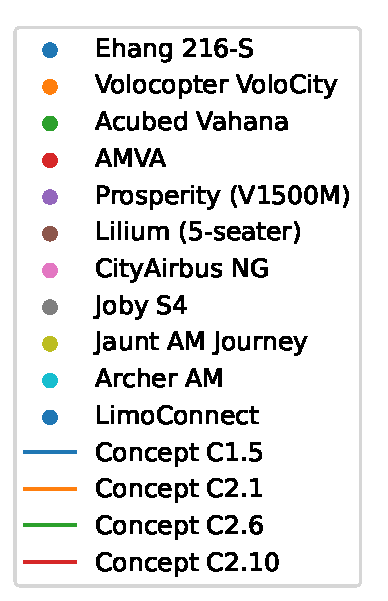
\includegraphics[width=\textwidth]{figures/VandV/legend}
        \caption{Legend}
        \label{fig:MassValidationLegend}
    \end{subfigure}
    \caption{Preliminary mass estimation compared to literature}
    \label{fig:MassValidation}
\end{figure}

To get a clearer picture of the effect of the payload mass and range on the total mass simultaneously, the total mass of Concept~\ref{C2.10} is shown in \Cref{fig:MassValidation2} for varying payload masses and ranges.
The total mass increases when moving to the right and upwards in the plot, which resonates with the expectations.
\begin{figure}[ht]
    \centering
    
\includegraphics[width=0.8\textwidth]{figures/VandV/C2.10_mass_over_payload_and_range}
    \caption{Total mass of concept \ref{C2.10} for varying payload mass and range, compared to literature data.}
    \label{fig:MassValidation2}
\end{figure}

\subsection{Validation of the Class II Sizing}\label{subsec:ValidationClassIISizing}
The mass breakdown diagrams of the different concepts (\Cref{fig:mass-breakdown}) are compared with the mass breakdown of a tilt-rotor aircraft from Kadhiresan et al.~\cite{Kadhiresan_Duffy_2019}.
The battery mass of the tilt-rotor aircraft is 25.7\% of the total mass, which is in line with the battery mass of the different concepts (26.0\% for Concept~\ref{C1.5}, 23.0\% for Concept~\ref{C2.1}, 25.2\% for Concept~\ref{C2.6}, and 24.0\% for Concept~\ref{C2.10}, as shown in \Cref{fig:mass-breakdown}).

Subcomponents of the Class II sizing tool are validated separately, where the engine mass estimation from \Cref{eq:m_motor_classII} is compared to literature data of electric motors in \Cref{fig:EngineValidation}.
The data points are taken from Ugwueze et al.~\cite{Ugwueze_Sizing_Method}, and the expected engine mass is within the range of the data.
\begin{figure}[H]
    \centering
    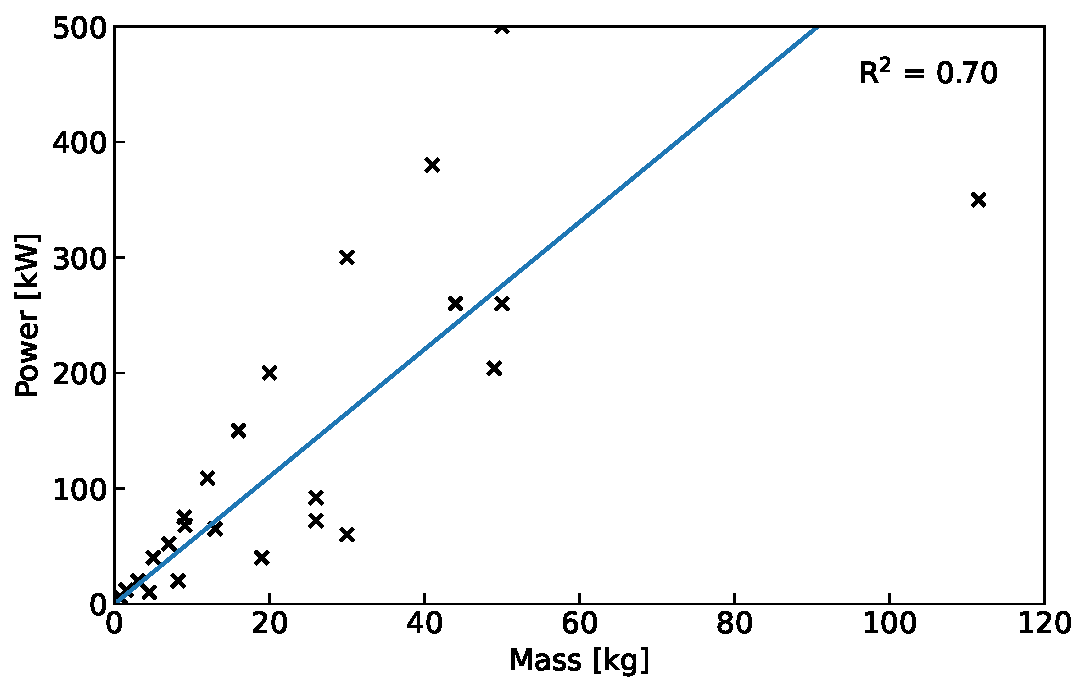
\includegraphics[width=0.7\textwidth]{figures/VandV/power_over_mass}
    \caption{Engine mass estimation from \Cref{eq:m_motor_classII} compared to literature data}
    \label{fig:EngineValidation}
\end{figure}

In the future, other subcomponents of the preliminary sizing tool should be validated as well.
The Class II model is also validated by validating the total mass model in \Cref{subsec:ValidationMassModel}.

\subsection{Validation of the Energy Consumption Model}\label{subsec:ValidationEnergyConsumptionModel}
The energy breakdown diagrams of the different concepts (\Cref{fig:energy-breakdown}) are compared with the energy analysis of the Joby aircraft from James Wang~\cite{weightperformanceslides}.
The Joby analysis contributes 86\% of the energy consumption to the cruise phase, 1.4\% to the take-off phase, and 8.3\% to the climb phase.
This is in line with the energy breakdown of the different concepts.
For instance, Concept~\ref{C1.5} has 82.5\% of the energy consumption in the cruise phase, 1.4\% in the take-off phase, and 10.7\% in the climb phase (\Cref{fig:energy-breakdown-C1.5}).
Only the climb energy of the model exceeds the Joby analysis, which is to be expected since the climb phase is modelled in a vertical configuration, as explained in \Cref{subsec:Class_II_sizing_Energy_System_Mass}.
Wang’s model uses cruise climb, which is more efficient than vertical climb.

\section{Future V\&V}\label{sec:VVProcedure}
For future verification and validation, the following steps are recommended:
\begin{itemize}
    \item More comparison to literature data for mass and energy breakdown.
    \item CAD model analysis, to compare the mass distribution of the concepts to the mass distribution of the CAD models.
    \item Computer simulations, to verify the energy consumption and asses the performance and stability of the concepts.
    \item The creation of a three-dimensional physical model to do testing in a real-world environment.
    \item Unit tests for the code base to verify the correctness of the code.
    \item Research and validate the hinge-loading based on current folding wing aircraft.
\end{itemize}